\documentclass[12pt]{article}
\usepackage[margin=1in]{geometry}
\usepackage{amsmath,amssymb}
\usepackage{graphicx}
\usepackage{booktabs}
\usepackage{siunitx}
\usepackage[colorlinks,citecolor=blue,urlcolor=blue]{hyperref}
\usepackage{natbib}
\bibliographystyle{unsrtnat}

\graphicspath{{../results/}}

\title{Kuramoto-coupled metachronal wave locomotion for pneumatic soft robots:
       simulation of three lobopodian morphologies}

\author{Carmen Mitchell$^{1,2}$\\
\small $^1$Department of Computer Science, Hunter College,
City University of New York, New York, NY 10065, USA\\
\small $^2$Division of Chemistry and Chemical Engineering,
California Institute of Technology, Pasadena, CA 91125, USA\\
\small \texttt{carmenm@caltech.edu}}

\date{}

\begin{document}
\maketitle

% ============================================================
\begin{abstract}
Multi-legged soft robots inspired by Onychophora (velvet worms) and
Cambrian lobopodians offer a promising locomotion paradigm for unstructured
benthic environments, yet the relationship between body morphology,
central pattern generator (CPG) parameters, and locomotion performance
remains poorly characterized.
We present a MuJoCo-based simulation study of three pneumatic lobopodian
robots (HALLU-S, HALLU-F, and HALLU-C) with 7, 9, and 25 leg pairs
respectively, each driven by a Kuramoto-coupled phase oscillator CPG
producing metachronal waves.
We systematically evaluate the effects of CPG frequency, coupling
strength, wave direction, phase noise, and incline angle on locomotion
metrics including speed, step length, gait quality, and cost of transport.
Key findings include: (i) retrograde metachronal waves produce 23--29\%
higher speeds than direct waves, consistent with biological observations
in \textit{Peripatus} (Manton, 1950);
(ii) moderate phase noise enhances locomotion speed by up to 119\%
through a stochastic resonance mechanism in the coupled oscillator
network;
(iii) inter-leg phase offsets follow the panarthropod $\phi_I = 1/2n$
scaling law, with root-mean-square tracking errors of
\SIrange{2.6}{4.8}{\degree} across morphologies.
These results establish design principles for CPG-driven soft robots
with high leg counts and provide simulation-validated parameters for
physical prototype development.
\end{abstract}

\paragraph{Keywords:} central pattern generator, metachronal wave,
soft robotics, Kuramoto oscillators, lobopodian, biomimetic locomotion,
stochastic resonance

% ============================================================
\section{Introduction}
\label{sec:intro}

Locomotion in multi-legged organisms relies on coordinated wave-like
patterns of leg activation known as metachronal waves
\citep{manton1950locomotory, manton1952evolution}.
Among extant panarthropods, Onychophora (velvet worms) represent a
particularly compelling model for soft-bodied multi-legged locomotion:
their unjointed lobopod legs, hydrostatic skeleton, and high leg counts
(13--43 pairs) produce robust walking gaits across irregular terrain
without the rigid kinematic constraints of arthropod limbs
\citep{oliveira2019functional, nirody2021universal}.

Soft robotics has seen rapid progress in design, fabrication, and
control \citep{rus2015design}, and recent reviews highlight growing
interest in multi-legged bio-inspired robots with flexible bodies
\citep{li2024bionic}.
Central pattern generators (CPGs) provide a biologically grounded
framework for controlling rhythmic locomotion in robots
\citep{ijspeert2008central}.
The Kuramoto model of coupled phase oscillators is particularly suited
to metachronal wave generation, as it guarantees frequency
synchronization while maintaining stable inter-oscillator phase
relationships through nearest-neighbor coupling
\citep{kuramoto1984chemical, strogatz2000kuramoto}.
Several groups have applied CPG control to hexapod and multi-legged
robots \citep{owaki2017quadruped, yasui2017decentralized}, and
recent work has demonstrated self-reconfigurable multi-legged swarms
for challenging terrain \citep{ozkanaydin2021selfreconfigurable},
but implementations with high leg counts ($n > 8$) and soft, compliant
bodies remain rare.

This paper presents a simulation study of three pneumatic soft robots
inspired by lobopodian body plans, ranging from 7 to 25 leg pairs.
Each variant is modeled in MuJoCo with physically realistic contact
mechanics, compliant body segments, and first-order pneumatic actuator
dynamics.
A Kuramoto-coupled CPG drives binary solenoid valves that inflate
and deflate each leg pair in a metachronal sequence.
We conduct five systematic analyses:
\begin{enumerate}
    \item Frequency sweep: speed, step length, and cost of transport
          as functions of CPG drive frequency
    \item Coupling gain sweep: effect of Kuramoto coupling strength $K$
          on gait synchronization
    \item Wave direction comparison: direct (anterior-to-posterior)
          versus retrograde (posterior-to-anterior) metachronal waves
    \item Noise robustness: locomotion performance under stochastic
          phase perturbations
    \item Incline performance: locomotion on slopes up to
          \SI{30}{\degree}
\end{enumerate}
Results are compared to biological data from \textit{Peripatus}
\citep{manton1950locomotory} and the panarthropod phase offset scaling
law \citep{nirody2021universal}.


% ============================================================
\section{Methods}
\label{sec:methods}

\subsection{Robot morphology}
\label{sec:morphology}

Three robot variants were modeled based on the body plans of extant and
extinct lobopodians (table~\ref{tab:variants}).
All variants share a common architecture: a segmented flexible body tube
(silicone analogue, density \SI{1100}{\kilogram\per\metre\cubed}) with
bilateral pairs of unjointed lobopod legs attached laterally to each
segment.
Body segments are connected by hinge joints with passive stiffness
($k = \SI{0.08}{\newton\metre\per\radian}$) and damping
($b = \SI{0.015}{\newton\metre\second\per\radian}$), constrained to
$\pm\SI{0.15}{\radian}$ in both pitch and yaw.
Legs are modeled as capsule geometries
(radius \SI{3}{\milli\metre}, length \SI{18}{\milli\metre} for S/F,
\SI{15}{\milli\metre} for C) with a single pitch-axis hinge
(range $[-0.3, 0.8]$~rad, $k = 0.02$, $b = 0.005$).

\begin{table}[ht]
\centering
\caption{Robot variant specifications. Phase offset is $\pi / n_v$
where $n_v$ is the number of valve groups.}
\label{tab:variants}
\begin{tabular}{lccc}
\toprule
Parameter & HALLU-S & HALLU-F & HALLU-C \\
\midrule
Biological model & \textit{H.\ sparsa} & \textit{H.\ fortis} & \textit{Carbotubulus} \\
Leg pairs & 7 & 9 & 25 \\
Valve groups & 7 & 9 & 8 \\
Body length (mm) & 120 & 150 & 300 \\
Segment length (mm) & 15.0 & 15.0 & 11.5 \\
Segments & 8 & 10 & 26 \\
Body mass (g) & 32.2 & 40.9 & 72.4 \\
Phase offset (deg) & 25.7 & 20.0 & 22.5 \\
\bottomrule
\end{tabular}
\end{table}

HALLU-C uses a valve zone architecture: 25 leg pairs are grouped into
8 pneumatic zones (3--3--3--3--3--3--3--4 legs per zone), each driven
by a single CPG oscillator.
This reflects the practical constraint that high-leg-count robots
require valve multiplexing to limit pneumatic hardware complexity.

\subsection{Simulation environment}
\label{sec:simulation}

Simulations were conducted in MuJoCo 3.9.0 \citep{todorov2012mujoco}
using the implicit Euler integrator with a timestep of \SI{2}{\milli\second}.
The ground plane uses a friction model with coefficients
$(\mu_s, \mu_d, \mu_r) = (1.0, 0.005, 0.001)$ for the floor and
$(1.5, 0.01, 0.01)$ for leg--ground contact (4-dimensional friction cone).
Each simulation runs for \SI{20}{\second} with the first
\SI{2}{\second} discarded as transient.

\subsection{Pneumatic actuator model}
\label{sec:actuator}

Each leg joint is driven by a general actuator modeling a binary
pneumatic solenoid valve.
The actuator applies force $F = g_a (u - q)$ where $g_a = 0.009$ is
the gain, $u \in [0, 1]$ is the control command, and $q$ is the joint
position.
First-order activation dynamics with time constant
$\tau = \SI{60}{\milli\second}$ model the pneumatic delay between valve
opening and leg inflation.

\subsection{CPG architecture}
\label{sec:cpg}

The CPG consists of $n$ Kuramoto-coupled phase oscillators, one per
valve group:
\begin{equation}
\dot{\theta}_i = 2\pi f + K \sum_{j \in \mathcal{N}(i)}
    \sin(\theta_j - \theta_i \mp \phi_0) + \sigma \xi_i(t)
\label{eq:kuramoto}
\end{equation}
where $f$ is the drive frequency, $K$ is the coupling gain,
$\phi_0 = \pi / n$ is the target inter-oscillator phase offset,
$\mathcal{N}(i) = \{i-1, i+1\}$ is the nearest-neighbor set, and
$\xi_i(t)$ is a unit-variance Wiener process with amplitude $\sigma$.
The sign convention in the coupling term determines wave direction:
the minus sign produces an anterior-to-posterior (direct) wave, while
the plus sign produces a posterior-to-anterior (retrograde) wave.

Each oscillator drives a binary valve command:
\begin{equation}
u_i = \begin{cases}
    1 & \text{if } \sin(\theta_i) > \cos(\pi d) \\
    0 & \text{otherwise}
\end{cases}
\label{eq:valve}
\end{equation}
where $d = 0.4$ is the duty cycle (fraction of the stride period
during which the valve is open).
Default parameters are $f = \SI{0.8}{\hertz}$ and $K = 2.0$.

\subsection{Metachronal wave coherence}
\label{sec:coherence}

We quantify the quality of the metachronal wave pattern using a
modified Kuramoto order parameter:
\begin{equation}
r = \left| \frac{1}{n} \sum_{i=1}^{n}
    \exp\!\big(j(\theta_i + i\,\phi_0)\big) \right|
\label{eq:coherence}
\end{equation}
where $r = 1$ indicates a perfect metachronal wave matching the target
phase offsets, and $r \to 0$ indicates desynchronization.

\subsection{Performance metrics}
\label{sec:metrics}

\paragraph{Speed.}
Mean forward speed computed from head sensor displacement during
steady-state locomotion.

\paragraph{Step length.}
Total displacement divided by the number of complete stride cycles,
where each cycle corresponds to one full rotation of the first
oscillator ($\Delta\theta_1 = 2\pi$).

\paragraph{Straightness.}
Ratio of net displacement to total path length, where 1.0 indicates
a perfectly straight trajectory.

\paragraph{Relative cost of transport.}
$\text{CoT} = \bar{u} / (m g v)$ where $\bar{u}$ is the
mean actuator command magnitude, $m$ is total body mass, $g$ is
gravitational acceleration, and $v$ is mean displacement speed.
This metric uses actuator commands as a power proxy and is valid only
for relative comparison between variants with identical actuator models.

\paragraph{Froude number.}
$\text{Fr} = v^2 / (g L)$ where $L$ is body length, providing a
dimensionless speed for comparison with biological organisms.

\subsection{Experimental protocol}
\label{sec:protocol}

All simulations are deterministic for a given set of initial conditions.
To quantify sensitivity to initial conditions, the frequency sweep
(section~\ref{sec:freq_sweep}) was repeated with three trials per
condition, each with independent random perturbations to the initial
oscillator phases ($\sigma_0 = \SI{0.05}{\radian} \approx
\SI{3}{\degree}$).
The noise robustness sweep (section~\ref{sec:noise}) inherently
includes stochastic variation and was run with three trials per noise
level.
The slope analysis uses signed forward displacement to correctly
capture backward sliding at steep inclines.


% ============================================================
\section{Results}
\label{sec:results}

\subsection{Phase-lag tracking}
\label{sec:phase_lag}

All three variants achieved stable metachronal wave patterns with
tight phase-lag tracking (figure~\ref{fig:phase}).
HALLU-S exhibited the best tracking performance with a root-mean-square
error (RMSE) of \SI{2.6}{\degree} relative to the coupling target of
\SI{-25.7}{\degree} (measured mean: \SI{-23.2}{\degree}).
HALLU-F showed an RMSE of \SI{4.8}{\degree} (target
\SI{-20.0}{\degree}, measured \SI{-15.4}{\degree}), and HALLU-C
achieved \SI{3.7}{\degree} (target \SI{-22.5}{\degree}, measured
\SI{-18.9}{\degree}).

The systematic undershoot of the phase lag target (measured offsets
2--5\si{\degree} less negative than the CPG target) arises from
ground reaction forces and body compliance, not from CPG dynamics.
The Kuramoto model predicts zero steady-state phase error when all
oscillators share the same natural frequency ($\Delta\omega = 0$),
which is the case here.
The observed deviation therefore reflects the mechanical coupling
between the body and the substrate, where ground contact forces during
the stance phase resist the phase advance commanded by the CPG.

\begin{figure}[ht]
\centering
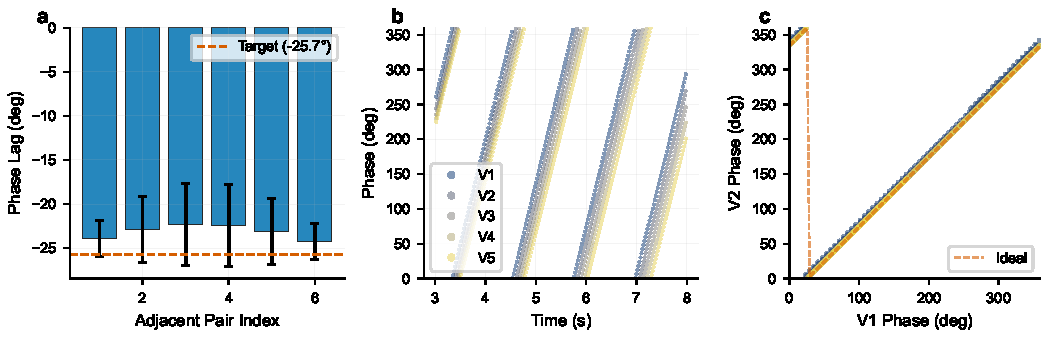
\includegraphics[width=\textwidth]{hallu-s_phase_analysis.pdf}
\caption{Phase-lag analysis for HALLU-S at $f = \SI{0.8}{\hertz}$,
$K = 2.0$.
(a) Mean inter-oscillator phase lag per adjacent pair (bars) with
standard deviation (error bars) and coupling target (dashed line).
(b) Phase trajectories of the first five oscillators showing stable
metachronal offset.
(c) Phase portrait ($\theta_1$ vs $\theta_2$) with ideal relationship
(dashed).}
\label{fig:phase}
\end{figure}

\subsection{Frequency sweep}
\label{sec:freq_sweep}

Speed increased monotonically with CPG frequency across all variants
(figure~\ref{fig:comparison}a), consistent with biological
speed--frequency scaling observed in \textit{Peripatus}
\citep{manton1950locomotory}.
At the baseline frequency of \SI{0.8}{\hertz}, HALLU-C (25 leg pairs)
achieved the highest speed (\SI{36.2 \pm 0.2}{\milli\metre\per\second}),
followed by HALLU-F (\SI{32.1 \pm 0.2}{\milli\metre\per\second}) and
HALLU-S (\SI{30.1 \pm 0.2}{\milli\metre\per\second}).
Standard deviations across three initial-condition perturbation trials
were consistently below \SI{0.6}{\milli\metre\per\second}, confirming
robustness to initial conditions.

Step length decreased with increasing frequency for HALLU-S and HALLU-F
(figure~\ref{fig:comparison}b), indicating that the speed increase is
driven primarily by stride frequency rather than stride amplitude.
Relative cost of transport decreased with frequency across all variants
(figure~\ref{fig:comparison}d), consistent with the reduced metabolic
cost per stride observed in biological multi-legged walkers at higher
speeds.

\begin{figure}[ht]
\centering
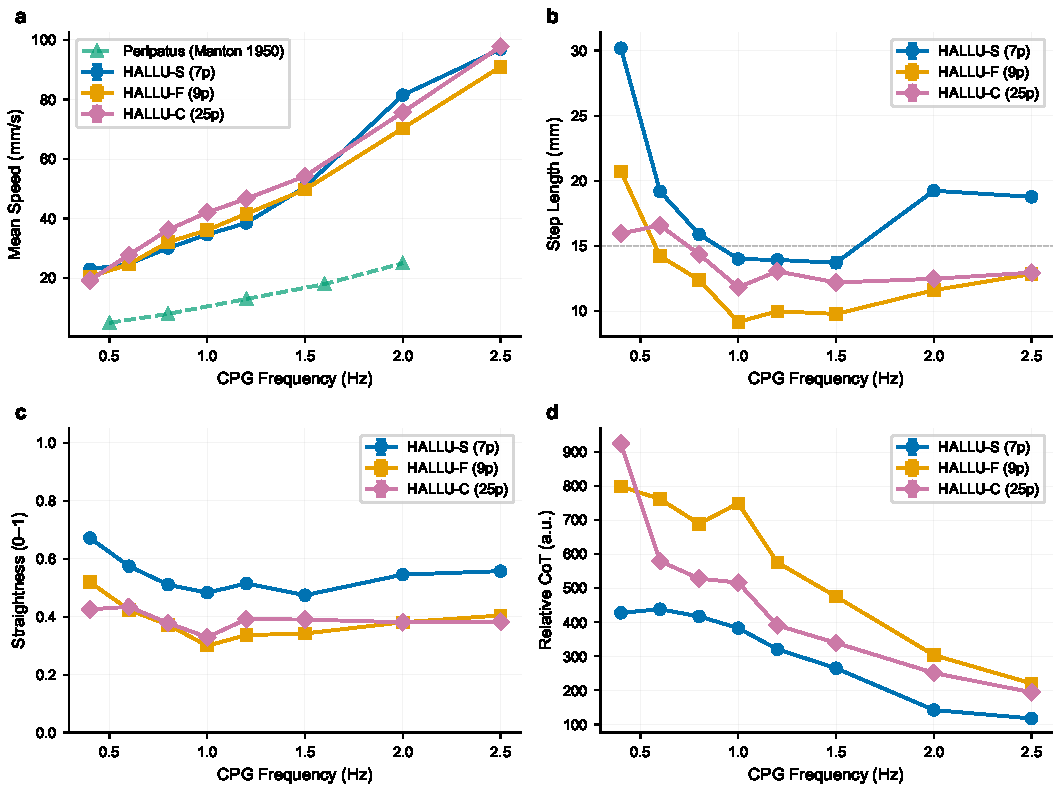
\includegraphics[width=\textwidth]{variant_comparison.pdf}
\caption{Locomotion metrics across CPG frequency for three morphologies.
Error bars show standard deviation over three trials with randomized
initial phase perturbation ($\sigma_0 = \SI{0.05}{\radian}$).
(a) Speed versus frequency, with \textit{Peripatus} data (Manton,
1950) for biological comparison.
(b) Step length.
(c) Path straightness.
(d) Relative cost of transport.}
\label{fig:comparison}
\end{figure}

\subsection{Coupling gain}
\label{sec:coupling}

Increasing the Kuramoto coupling gain $K$ from 0.5 to 6.0 produced a
monotonic decrease in speed (from \SI{43.2}{\milli\metre\per\second} to
\SI{27.2}{\milli\metre\per\second} for HALLU-S) but a monotonic
increase in path straightness (0.30 to 0.61) and step length
(figure~\ref{fig:coupling}).
This reflects a fundamental trade-off in coupled oscillator CPGs:
stronger coupling enforces tighter phase synchronization, producing
more coherent gaits with less lateral drift, but the rigid phase
relationships constrain the body dynamics and reduce speed.
The design value of $K = 2.0$ represents a compromise between gait
quality and locomotion speed.

\begin{figure}[ht]
\centering
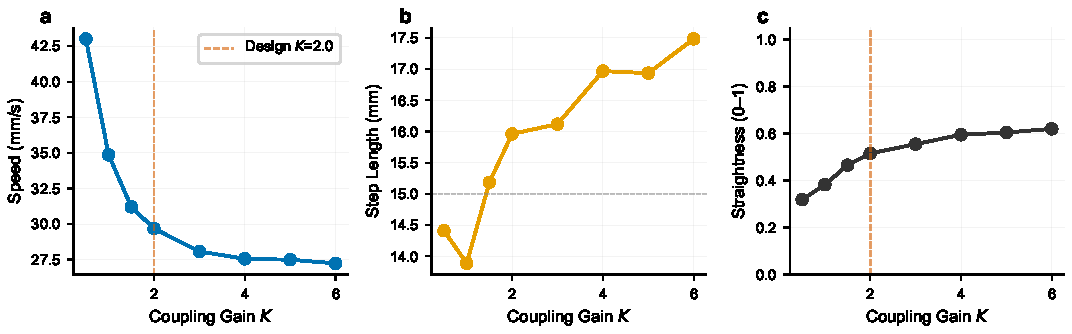
\includegraphics[width=\textwidth]{coupling_analysis.pdf}
\caption{Effect of Kuramoto coupling gain $K$ on HALLU-S locomotion
at $f = \SI{0.8}{\hertz}$.
(a) Speed decreases with coupling strength.
(b) Step length increases above $K \approx 2$.
(c) Path straightness improves with stronger phase locking.
Dashed line: design value $K = 2.0$.}
\label{fig:coupling}
\end{figure}

\subsection{Wave direction}
\label{sec:wave_direction}

Retrograde metachronal waves (posterior-to-anterior activation)
produced higher speeds than direct waves (anterior-to-posterior)
for HALLU-S (+29\%, from 29.7 to \SI{38.4}{\milli\metre\per\second})
and HALLU-F (+23\%, from 32.5 to \SI{40.0}{\milli\metre\per\second})
(figure~\ref{fig:wave_dir}).
HALLU-C showed negligible difference between wave directions
($< 1\%$), likely because its valve zone architecture (3--4 legs per
zone) averages out the directional effect within each zone.

This result independently reproduces the biological observation by
\citet{manton1950locomotory} that \textit{Peripatus} employs retrograde
metachronal waves for forward locomotion.
The speed advantage of retrograde waves arises because the
posterior-to-anterior activation sequence produces ground reaction
forces that constructively sum in the forward direction: each leg
pushes backward during its power stroke while the leg anterior to it
is in recovery, creating a net forward thrust that propagates along
the body.

\begin{figure}[ht]
\centering
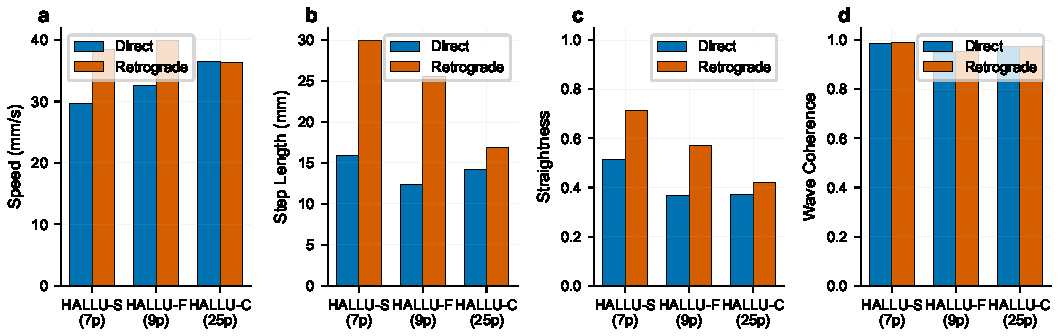
\includegraphics[width=\textwidth]{wave_direction_comparison.pdf}
\caption{Direct versus retrograde metachronal wave comparison at
$f = \SI{0.8}{\hertz}$, $K = 2.0$.
(a) Speed, (b) step length, (c) path straightness, (d) wave coherence.
Retrograde waves produce 23--29\% higher speeds for HALLU-S and HALLU-F.}
\label{fig:wave_dir}
\end{figure}

\subsection{Noise robustness and stochastic resonance}
\label{sec:noise}

Moderate phase noise dramatically enhanced locomotion performance
(figure~\ref{fig:noise}).
For HALLU-S, speed increased from
\SI{29.7}{\milli\metre\per\second} at $\sigma = 0$ to a peak of
\SI{65.0}{\milli\metre\per\second} at $\sigma = 7.0$~rad/$\sqrt{s}$,
a 119\% increase.
Similar peaks were observed for HALLU-F (85\% increase) and HALLU-C
(85\% increase), all peaking near $\sigma = 7.0$.
Beyond this optimum, speed degraded as the noise amplitude overwhelmed
the coupling and destroyed the metachronal wave pattern (wave
coherence $r < 0.3$ for $\sigma > 15$).

This noise-enhanced performance constitutes stochastic resonance in the
coupled oscillator network \citep{gammaitoni1998stochastic}.
The mechanism is as follows: at $\sigma = 0$, the deterministic CPG
locks into a fixed phase relationship that, due to body--ground
mechanical coupling, does not perfectly match the optimal locomotion
phase pattern.
Moderate noise explores the basin of attraction around the CPG fixed
point, transiently visiting phase configurations that interact more
favorably with the ground contact dynamics.
The result is a higher time-averaged speed despite (or rather because
of) the phase variability.
At excessive noise, the oscillators desynchronize entirely and
coordinated locomotion collapses.

Path straightness showed a complementary pattern: it peaked at low
noise, declined moderately through the stochastic resonance regime,
and collapsed above $\sigma = 10$.
Wave coherence decreased monotonically with noise amplitude, confirming
that the speed enhancement does not arise from improved wave quality
but from dynamical exploration of the phase space.

\begin{figure}[ht]
\centering
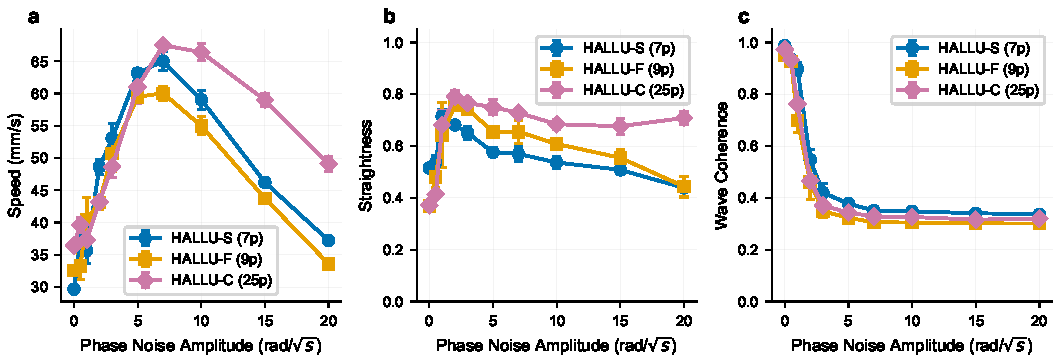
\includegraphics[width=\textwidth]{noise_robustness.pdf}
\caption{CPG noise robustness sweep.
(a) Speed versus phase noise amplitude, showing stochastic resonance
peak near $\sigma = 7.0$~rad/$\sqrt{s}$.
(b) Path straightness degrades gradually with noise.
(c) Kuramoto wave coherence decreases monotonically.
Error bars: standard deviation over three trials.}
\label{fig:noise}
\end{figure}

\subsection{Incline performance}
\label{sec:slope}

Forward speed decreased approximately linearly with slope angle up
to \SI{15}{\degree}, beyond which all variants exhibited net backward
sliding (figure~\ref{fig:slope}a).
The critical angle (zero net forward speed) was approximately
\SI{13}{\degree} for HALLU-S, \SI{15}{\degree} for HALLU-F, and
\SI{14}{\degree} for HALLU-C.
Cost of transport peaked sharply at angles just below the critical
angle (figure~\ref{fig:slope}b), reflecting the high actuator effort
required to maintain position against gravity with minimal forward
progress.
Path straightness was largely unaffected by slope up to
\SI{15}{\degree}, then declined as gravitational forces began to
dominate leg thrust (figure~\ref{fig:slope}c).

\begin{figure}[ht]
\centering
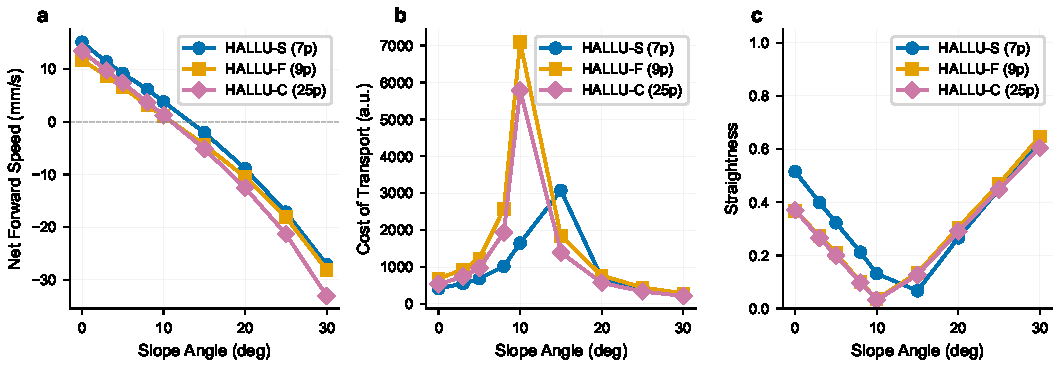
\includegraphics[width=\textwidth]{slope_performance.pdf}
\caption{Incline locomotion performance.
(a) Net forward speed versus slope angle; negative values indicate
backward sliding.
(b) Relative cost of transport peaks near the critical angle.
(c) Path straightness.}
\label{fig:slope}
\end{figure}

\subsection{Biological comparison}
\label{sec:bio_comparison}

The measured inter-leg phase offsets for all three variants fall on the
$\phi_I = 1/2n$ curve (figure~\ref{fig:bio}a), consistent with the
half-wavelength metachronal wave produced by the $\pi/n$ CPG offset.
This places our robots below the full-wavelength $\phi_I = 1/n$
scaling observed in biological panarthropods \citep{nirody2021universal},
reflecting a design choice rather than a tracking failure: our CPG
generates a half-body-length wave whereas biological organisms
typically produce full-body-length waves.

Speed--frequency scaling (figure~\ref{fig:bio}b) shows that all three
variants exceed \textit{Peripatus} speeds at frequencies above
\SI{0.6}{\hertz}, reaching 3--4$\times$ biological speeds at
\SI{2.5}{\hertz}.
When normalized by body length (figure~\ref{fig:bio}c), HALLU-S
achieves approximately 0.3~BL/s at \SI{1}{\hertz}, comparable to
\textit{Peripatus} at the same stride frequency.

\begin{figure}[ht]
\centering
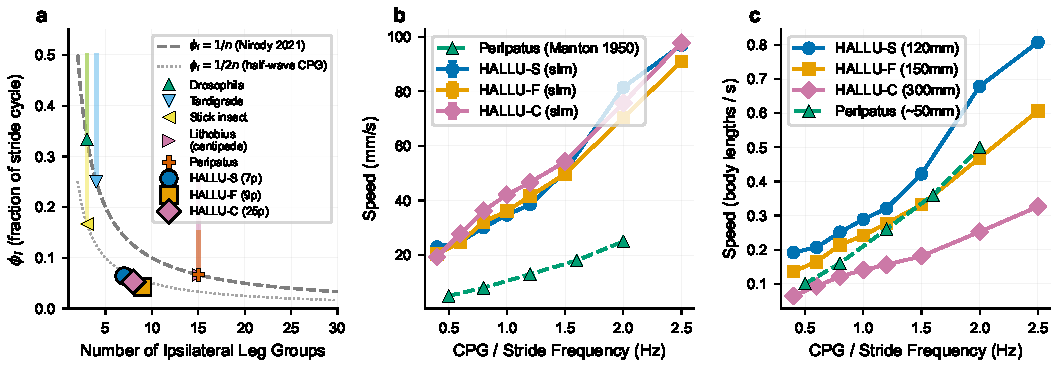
\includegraphics[width=\textwidth]{bio_comparison.pdf}
\caption{Biological comparison.
(a) Phase offset scaling: simulation data (large markers) against the
panarthropod $\phi_I = 1/n$ law (Nirody et al., 2021) and biological
data points.
Vertical bars indicate phase offset range from low to high speed.
(b) Speed versus stride frequency with \textit{Peripatus} reference
data (Manton, 1950).
(c) Size-normalized speed in body lengths per second.}
\label{fig:bio}
\end{figure}


% ============================================================
\section{Discussion}
\label{sec:discussion}

\subsection{Design implications}

The results establish several design principles for CPG-driven soft
robots with high leg counts:

\paragraph{Retrograde waves.}
The consistent superiority of retrograde metachronal waves for forward
locomotion (section~\ref{sec:wave_direction}) suggests that CPG
implementations for lobopodian robots should default to
posterior-to-anterior wave propagation.
This aligns with biological Onychophora and provides a 23--29\% speed
advantage at no additional hardware cost.

\paragraph{Noise tolerance.}
The stochastic resonance effect (section~\ref{sec:noise}) has practical
implications for pneumatic soft robots, where valve timing jitter from
pressure fluctuations, microcontroller latency, and sensor noise is
unavoidable.
Our results suggest that moderate timing imprecision may actually
\emph{improve} locomotion performance, relaxing the precision
requirements for embedded CPG implementations.

\paragraph{Valve zone grouping.}
The HALLU-C valve zone architecture demonstrates that high-leg-count
robots can use valve multiplexing ($\leq 8$ valve groups for 25 leg
pairs) without sacrificing locomotion speed.
However, the loss of wave direction sensitivity
(section~\ref{sec:wave_direction}) suggests that finer-grained valve
control would be beneficial if the pneumatic hardware budget permits.

\paragraph{Coupling strength trade-off.}
The coupling gain $K$ controls a fundamental trade-off between speed
and gait quality (section~\ref{sec:coupling}).
For applications requiring straight-line traversal (e.g., pipeline
inspection), higher $K$ values are appropriate; for maximum speed
(e.g., rapid response), lower $K$ may be preferable.

\subsection{Limitations}

This study uses simulation exclusively; physical prototype validation
is ongoing and will be reported separately.
The pneumatic actuator model uses a simplified first-order dynamics
approximation that does not capture nonlinear effects such as flow
saturation, tube compliance, or pressure-dependent force output.
The relative cost of transport uses actuator commands as a power proxy
rather than measured mechanical power, and is therefore valid only for
relative comparison between variants with identical actuator parameters.
Biological reference data from \citet{manton1950locomotory} are
approximate values derived from 1950s cinematography and should be
interpreted with corresponding uncertainty.

The stochastic resonance finding requires careful interpretation: the
speed enhancement occurs at noise levels that degrade wave coherence,
suggesting that the mechanism involves dynamical exploration of the
phase space rather than improved coordination.
Whether this effect persists in physical systems with additional
sources of variability (ground irregularity, pneumatic pressure
fluctuations) remains an open question for experimental validation.


% ============================================================
\section{Conclusion}
\label{sec:conclusion}

We presented a systematic simulation study of Kuramoto-coupled CPG
locomotion for three pneumatic lobopodian soft robots with 7, 9, and
25 leg pairs.
The CPG achieves stable metachronal wave patterns with phase-lag
tracking errors of \SIrange{2.6}{4.8}{\degree}, retrograde waves
provide a 23--29\% speed advantage consistent with biological
observations, and a stochastic resonance mechanism produces up to
119\% speed enhancement under moderate phase noise.
These results provide simulation-validated design parameters and
control strategies for multi-legged soft robots, with physical
prototype fabrication and testing planned as the next phase of this
work.


% ============================================================
\section*{Data availability}

Simulation code, MuJoCo models, and all data files are available at
\url{https://github.com/venticedlatte/hallucigenia-cpg}.

\section*{Acknowledgments}

This work was supported by the John P.\ McNulty Scholars Program
and the Yalow Scholars Program at Hunter College, City University
of New York.

% ============================================================
\bibliography{references}

\end{document}
